\documentclass[a4paper,12pt]{book}
\usepackage{graphicx}
\usepackage[export]{adjustbox}
\usepackage{subcaption}
\graphicspath{{Pics/}}
\usepackage{charter}
\usepackage{fancyhdr}
\usepackage{enumerate}
\usepackage{enumitem}
\usepackage{siunitx}
\usepackage{amssymb}
\usepackage{longtable}
\usepackage{multicol}
\usepackage{multirow}
\usepackage{hhline}
\usepackage{parskip}
\setlength{\parskip}{6pt}
\usepackage{ragged2e}
\usepackage{geometry} %margin
\geometry{left=2.1cm,right=2.1cm,top=3cm,bottom=3cm}
\usepackage{setspace}
\SetSinglespace{1.2}
\singlespacing
\renewcommand{\ttfamily}{\fontfamily{pcr}\selectfont}
%\renewcommand{\familydefault}{\rmdefault}

\usepackage[,table]{xcolor}
\definecolor{LightBlue}{cmyk}{0.16,0.03,0.04,0}
\definecolor{Title}{cmyk}{0.8,0.1,0,0.3}
\setlength{\arrayrulewidth}{0.3mm}
\setlength{\tabcolsep}{2pt}
\setlength{\headheight}{15pt}
\renewcommand{\arraystretch}{1}
\usepackage{tikz}
\usepackage{nicematrix}
\newcommand*\circled[1]{\tikz[baseline=(char.base)]{\node[shape=circle,draw,inner sep=1pt] (char) {#1};}}

\newcolumntype{s}{>{\columncolor{Title}\RaggedLeft} m{3.5em}} % columntype for chapter title
\newcolumntype{d}{>{\columncolor{LightBlue}\RaggedRight} m{\textwidth}} % columntype for code bloc
\newcolumntype{a}{>{\columncolor{LightBlue}\RaggedRight} m{0.96\textwidth}} % columntype for secondary code bloc

\usepackage{titlesec}
\usepackage[hidelinks]{hyperref}
\urlstyle{same}

\captionsetup[figure]{labelsep=period,font={bf}}
\captionsetup[table]{font={bf},labelsep=period}

\newcommand{\titlename}{}

\newcommand{\chaptertitle}[2]{ %reset chapter format
\vspace{-120pt}
\gdef\titlename{#1}
{
\SetSinglespace{1.1}
\singlespacing
\Huge\bfseries
\setlength{\tabcolsep}{8pt}
\renewcommand{\arraystretch}{1.5}
\begin{tabular}{s >{\RaggedRight}m{14.5em}}
\textcolor{white}{Chapter\newline\thechapter}&\textcolor{Title}{#2}
\end{tabular}
}
}

\newcommand{\partpic}[1]{%insert picture
    \tikz[remember picture,overlay] \node at (current page.center){\includegraphics[width=\paperwidth]{#1}};
}

\titleformat{\part} %reset part %format
{\huge\bfseries} % format
{} % label
{0em} % sep
{\Centering} % before-code

\titleformat{\chapter} %reset chapter %format
{\huge\bfseries} % format
{} % label
{0em} % sep
{\Centering} % before-code
\titlespacing{\chapter}{0pt}{0pt}{0pt}

\titleformat{\section} %reset section %format
{\Large\bfseries} % format
{\textcolor{Title}{\thesection}} % label
{0.5em} % sep
{\color{Title}} % before-code
\titlespacing{\section}{0pt}{12pt}{6pt}

\titleformat{\subsection} %reset subsection %format
{\large\bfseries} % format
{\textcolor{Title}{\thesubsection}} % label
{0.5em} % sep
{\color{Title}} % before-code
\titlespacing{\subsection}{0pt}{8pt}{6pt}

\newenvironment{term}[1]{
    \textbf{#1}

    \leftskip 1em
    \parskip 0pt
}

\newenvironment{secterm}[1]{
    \textbf{#1}

    \leftskip 2em
    \parskip 0pt
}

\newenvironment{codebloc}{ %define code bloc style
    \ttfamily\footnotesize
    \renewcommand{\arraystretch}{1}
}

\newcommand{\note}[2][NOTE]{ %Note/Tips
\vspace{6pt}
\begin{tabular}{b{\textwidth}}
\hline
\fontfamily{phv}\selectfont \textbf{#1}\\
\leftskip 1em #2\\
\hline
\end{tabular}
}

\newcommand{\secnote}[2][NOTE]{ %Note/Tips
\vspace{6pt}
\begin{tabular}{b{0.93\textwidth}}
\hline
\fontfamily{phv}\selectfont \textbf{#1}\\
\leftskip 1em #2\\
\hline
\end{tabular}
}

\title{ESP32-C3 Wireless Adventure\par \Large A comprehensive guide to IoT}
\author{Espressif Systems}
\date{\today}

\pagestyle{fancy} % reset head&foot
\fancyhead{} % clear all header fields
\renewcommand\headrulewidth{0pt}
\fancyfoot{} % clear all footer fields
\setcounter{chapter}{13}

\begin{document}

\fancyfoot[LE]{\fontfamily{cmss}\selectfont{\textbf{\thepage} \ \textit{ESP32-C3 Wireless Adventure: A comprehensive guide to IoT}}}
\fancyfoot[RO]{\fontfamily{cmss}\selectfont{\textit{Chapter \thechapter. \titlename} \ \textbf{\thepage}}}

\chapter[Firmware Burning and Testing for Mass Production]{\chaptertitle{Firmware Burning and Testing for Mass Production}{Firmware Burning and Testing for Mass Production}}

\vspace{36pt}
After the development stage, it is time for pilot-run verification tests and mass production. Pilot-run verification tests include:

\begin{term}{EVT (Engineering Verification Test)}
An EVT is performed on the first PCBA (Printed Circuit Board Assembly) to ensure that basic designs meet requirements and specifications, including basic hardware functions, RF performance, RF interference, and power consumption. The EVT process may iterate as many times as required to identify and fix all the issues.
\end{term}

\begin{term}{DVT (Design Verification Test)}
A DVT is performed on the whole product to ensure that the product meets requirements and specifications before moving towards mass production. DVT includes high/low temperature test, electrostatic discharge (ESD) test, and drop test.
\end{term}

\begin{term}{Product Certification}
Once the product passes EVT and DVT, a prototype can be prepared for national or alliance certifications, such as SRRC, FCC, CE, etc.
\end{term}

After trial production, the product is ready for mass production. Mass production involves many stages, such as material preparation, mounting, burning, testing, packaging, etc. This chapter only focuses on two stages that are closely related to Espressif's products - firmware burning and product testing.

\section{Firmware Burning in Mass Production}

Firmware for mass production mainly includes two parts: application firmware and data partitions. This section focuses on defining the application firmware and data partitions and how to flash them.

\subsection{Defining Data Partitions}

To identify different smart products on the market and bind them to their users, it is often necessary to store some unique data in each smart product. For example, in order for smart products to effectively connect to the vendor's cloud platform, unique authentication information (e.g., device certificate, ID, and password) should be generated and stored in each smart product. It will be used on the server side when the smart product is connected and authenticated.

During the development stage, we can easily store the authentication information in a smart product, by defining constants and storing them in firmware, or by writing it into Flash. But in mass production, these methods become clumsy and inefficient. Therefore, a more convenient method is needed to burn data partitions in actual production.

In \textit{Part II Hardware and Driver Development}, Section 6.4.1, we introduced the NVS library, which can be an option to store the unique mass production data of smart products, as well as any application-related user data. User data are often read and modified when using a smart production, and will be erased when reset to factory, while the unique mass production data can only be read. Therefore, mass production data and user data need to be assigned different namespaces, for example \texttt{mass\_prod} (for production data) and \texttt{user\_data} (for user data). This makes it possible to directly erase the user data while keeping the mass production data unaffected during a factory reset. Besides, the mass production data and user data can also be stored separately in different NVS partitions.

The following code shows how to store product certificate under \texttt{mass\_prod} and the SSID of Wi-Fi under \texttt{user\_data}:

\begin{codebloc}
\begin{tabular}{d}
\vspace{2pt}
\begin{verbatim}
1.  nvs_handle_t mass_prod_handle = NULL;
2.  nvs_handle_t user_data_handle = NULL;
3.  //Initialize NVS Flash Storage
4.  nvs_flash_init_partition(partition_label);
5.  
6.  //Open non-volatile storage with mass_prod namespace
7.  nvs_open("mass_prod", NVS_READONLY, &mass_prod_handle);
8.  
9.  //Open non-volatile storage with user_data namespace
10. nvs_open("user_data", NVS_READWRITE, &user_data_handle);
11. 
12. uint8_t *product_cert = malloc(2048);
13. //read operation in mass_prod namespace
14. nvs_get_blob(mass_prod_handle, "product_cert", &product_cert);
15. 
16. char ssid[36] = {0};
17. //read operation in user_data namespace
18. nvs_get_str(user_data_handle, "ssid", &ssid);
19. //write operation in user_data namespace
20. nvs_set_str(user_data_handle, "ssid", &ssid);
21. 
22. //Erase user_date namespace when reset to factory
\end{verbatim}
\verb|23. nvs_erase_all(user_data_handle);|
\end{tabular}
\end{codebloc}


Now that we’ve known how to store mass production data, we need to convert them into a required format before flashing them onto the device. The basic steps for generating mass production data are shown in Figure 14.1.
\begin{figure}[ht]
    \centering
    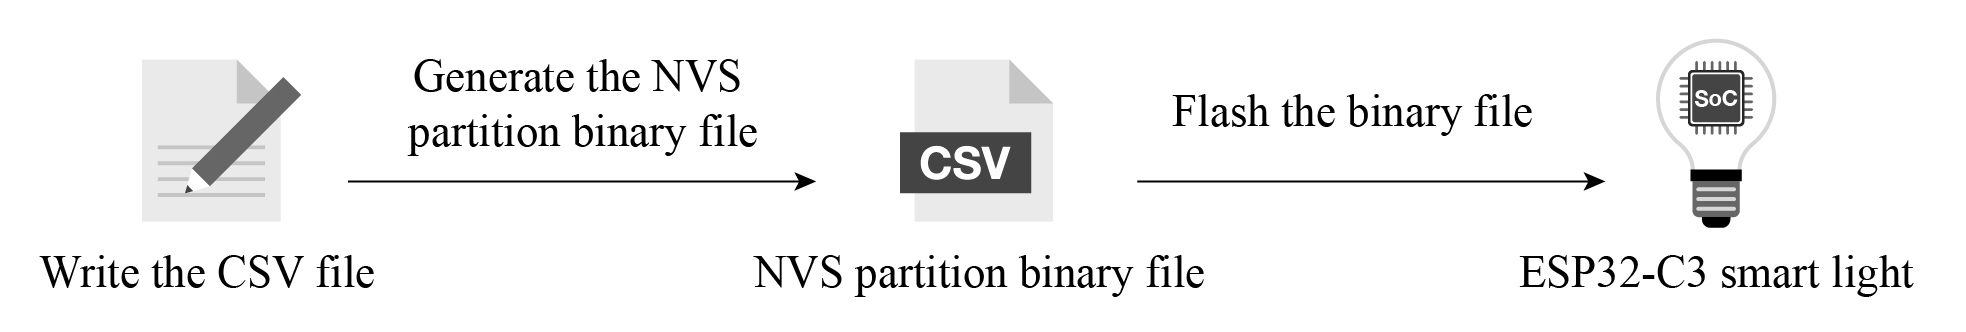
\includegraphics[width=\textwidth]{D14Z/14-1}
    \caption{Basic steps for generating mass production data}
\end{figure}

First, create a CSV file to store key-value pairs; write the data needed into the file. For mass production, an NVS partition binary file should be generated from this CSV file, then be burned to the device. For each device produced, a unique NVS partition binary file will be burned to it. For example:

\begin{codebloc}
\begin{tabular}{d}
\vspace{2pt}
\begin{verbatim}
1.  key,          type,     encoding, value
2.  mass_prod,    namespace,,
3.  ProductID,    data,     string,   12345
4.  DeviceSecret, data,     string,   12345678901234567890123456789012\end{verbatim}
\verb|5.  DeviceName,   data,     string,   123456789012|
\end{tabular}
\end{codebloc}


Second, use \texttt{esp-idf/components/nvs\_flash/nvs\_partition\_generator/nvs\_\\
partition\_gen.py} to generate the NVS partition binary file on the development host with the following command:

\begin{codebloc}
\begin{tabular}{d}
\$ \bfseries python \$IDF\_PATH/components/nvs\_flash/nvs\_partition\_generator/nvs\_partition\_\newline gen.py --input\ mass\_prod.csv --output mass\_prod.bin --size NVS\_PARTITION\_SIZE
\end{tabular}
\end{codebloc}

\note{Replace the \texttt{NVS\_PARTITION\_SIZE} parameter with the actual size of the corresponding NVS partition in the partition table. After executing the above command, the resulting file \texttt{mass\_prod.bin} is the binary file for mass production. Run the following command to burn this file to the device Flash.}

\begin{codebloc}
\begin{tabular}{d}
\$ \bfseries python \$IDF\_PATH/components/esptool\_py/esptool/esptool.py --port \$ESPPORT write\_flash NVS\_PARTITION\_ADDRESS mass\_prod.bin
\end{tabular}
\end{codebloc}

\note{Replace the \texttt{NVS\_PARTITION\_ADDRESS} parameter with the actual address of the corresponding NVS partition in the partition table.}

\subsection{Firmware Burning}

In mass production, the binary files that need to be burned to the device include:

\begin{itemize}
    \leftskip 1em
    \item firmware for mass production devices
    \setlength{\parskip}{0pt}
    \item binary files of mass production data
\end{itemize}

During the burning, it is necessary to ensure that a unique binary file of mass production data is burned to each device, while the application firmware is usually the same for all devices. To achieve this, we can write a script to generate a unique binary file of mass production data for each device based on its MAC address. Then, this file can be burned to the device together with the application firmware. In this process, a table that relates the MAC address of each device to its mass production data can also be created for querying, debugging, and tracking.

Espressif can customize firmware for our module products based on customers’ requirements. For example, we can conduct safety configurations to ESP32-C3 series of modules, including the unique mass production data for each device. In this way, Espressif modules can be mounted directly onto the product’s hardware circuit, which saves manufacturers’ trouble for secondary burning. Espressif also provides a Flash Download Tool, where a factory mode can be used to burn multiple devices at a time. For more details about the Flash Download Tool, please check the documentation on our website.
\begin{figure}[h!]
    \centering
    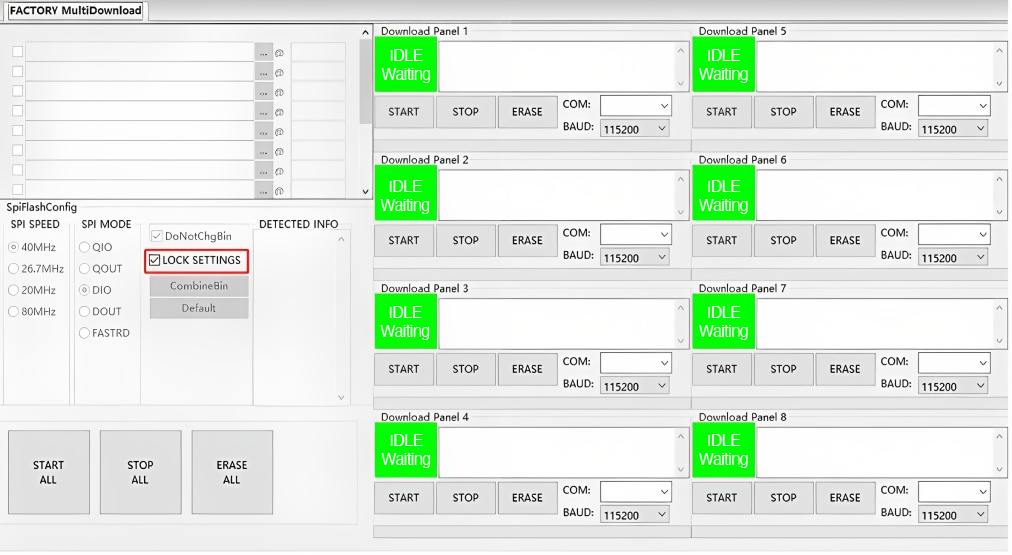
\includegraphics[width=0.7\textwidth]{D14Z/14-2}
    \caption{Interface of factory mode in Flash Download Tool}
\end{figure}

The interface of factory mode in the Flash Download Tool is shown in Figure 14.2. In factory mode, Flash Download Tool loads firmware through relative paths and by default burns the firmware stored in bin directory to device. Users may store their firmware in the bin folder under the tool directory so that they can copy the project to different computers without triggering path-related errors.

\section{Mass Production Testing}

The purpose of mass production testing is to ensure that the functions and performance of the whole product meet standards, so it is necessary to fully check the functions and performance of each product during this stage. Depending on the product characteristics, the schemes for mass production testing can be slightly different. For RF communication products, it is necessary to ensure that RF performance meets standards and each component functions as expected. This normally involves RF performance test, power consumption test, and functional test of various peripherals.

For wireless products, common mass production testing includes electromagnetic compatibility (EMC) test, RF performance test, production compliance test, safety test, SAR (Specific Absorption Rate) test, etc., among which the RF performance test is of high importance, thus requiring a large amount of testing. It is conducted to verify whether the RF performance of a product meets the designated requirements and relevant standards. It involves two sets of indicators: Transmitter (TX) and Receiver (RX) characteristics.

This section mainly introduces the mass production testing schemes for products with Espressif Wi-Fi / Bluetooth Low Energy (BLE) modules and chips, which can be used as a reference for designing testing schemes for similar products. For detailed information, please refer to Espressif Production Testing Guide on our official website. Generally, there are two production testing schemes available for RF performance test: \textbf{RF General- purpose Tester Scheme} (widely adopted in the industry) and \textbf{Signal Board Scheme} (designed by Espressif).

\begin{term}{RF General-purpose Tester Scheme}
The tester scheme is widely used for the production testing of Wi-Fi / BLE products. Espressif provides the necessary serial port commands and firmware, so the customers can easily use this scheme for testing. The testing steps are demonstrated in Figure 14.3.
\end{term}
\begin{figure}[h!]
    \centering
    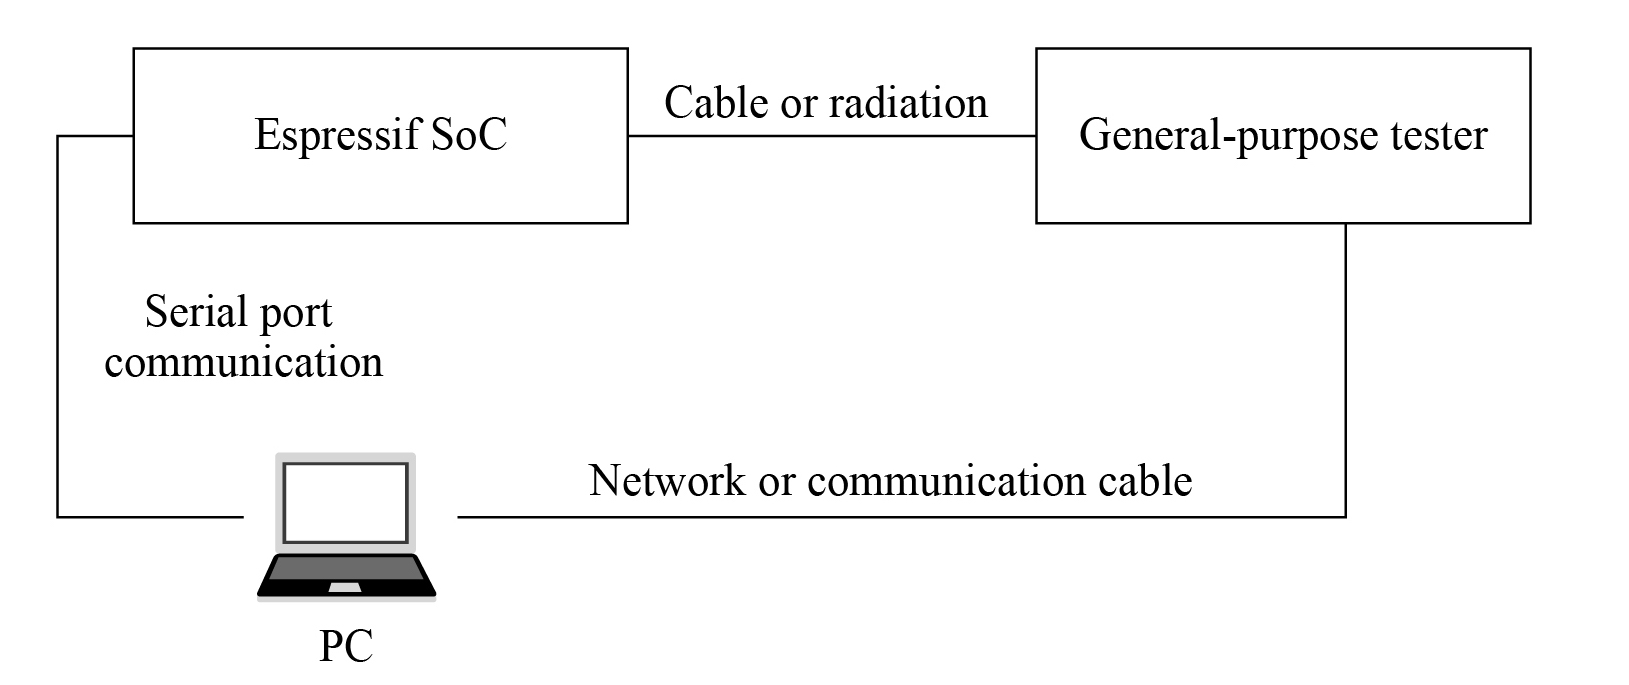
\includegraphics[width=0.8\textwidth]{D14Z/14-3}
    \caption{Diagram of the tester scheme}
\end{figure}

\begin{term}{Signal Board Scheme}
The signal board scheme is specially designed by Espressif, which can effectively test the RF performance of the mass-produced Wi-Fi / BLE products, thus guaranteeing the RF quality. This scheme features low cost of hardware and easy environment setup for factories.

\parskip 6pt
As demonstrated in Figure 14.4, the signal board can be used as a standard device to communicate with the DUT (Device Under Test) and test it by analyzing the communication data. Hardware connection for signal board scheme is demonstrated in Figure 14.5.
\end{term}

\begin{figure}[!h]
  \Centering
  \begin{minipage}[b]{0.45\textwidth}
    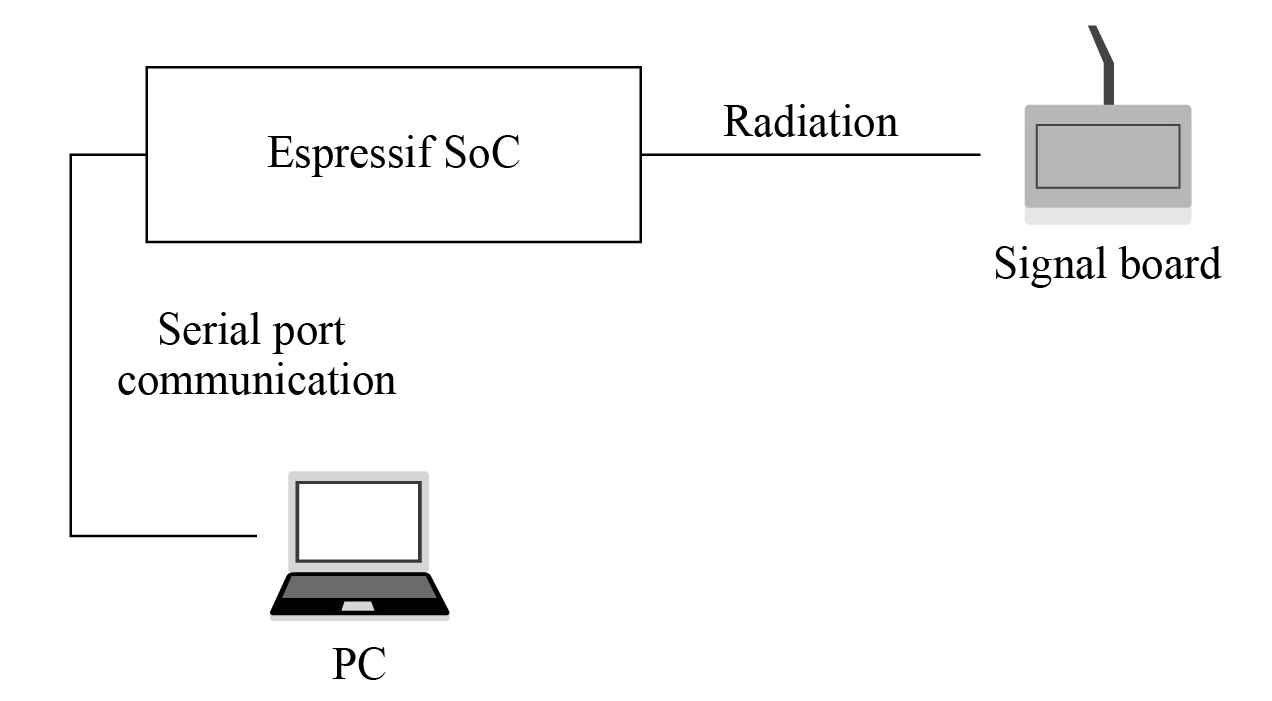
\includegraphics[width=\textwidth]{D14Z/14-4}
    \caption{\Centering\newline Diagram of signal board scheme}
  \end{minipage}
  \begin{minipage}[b]{0.53\textwidth}
    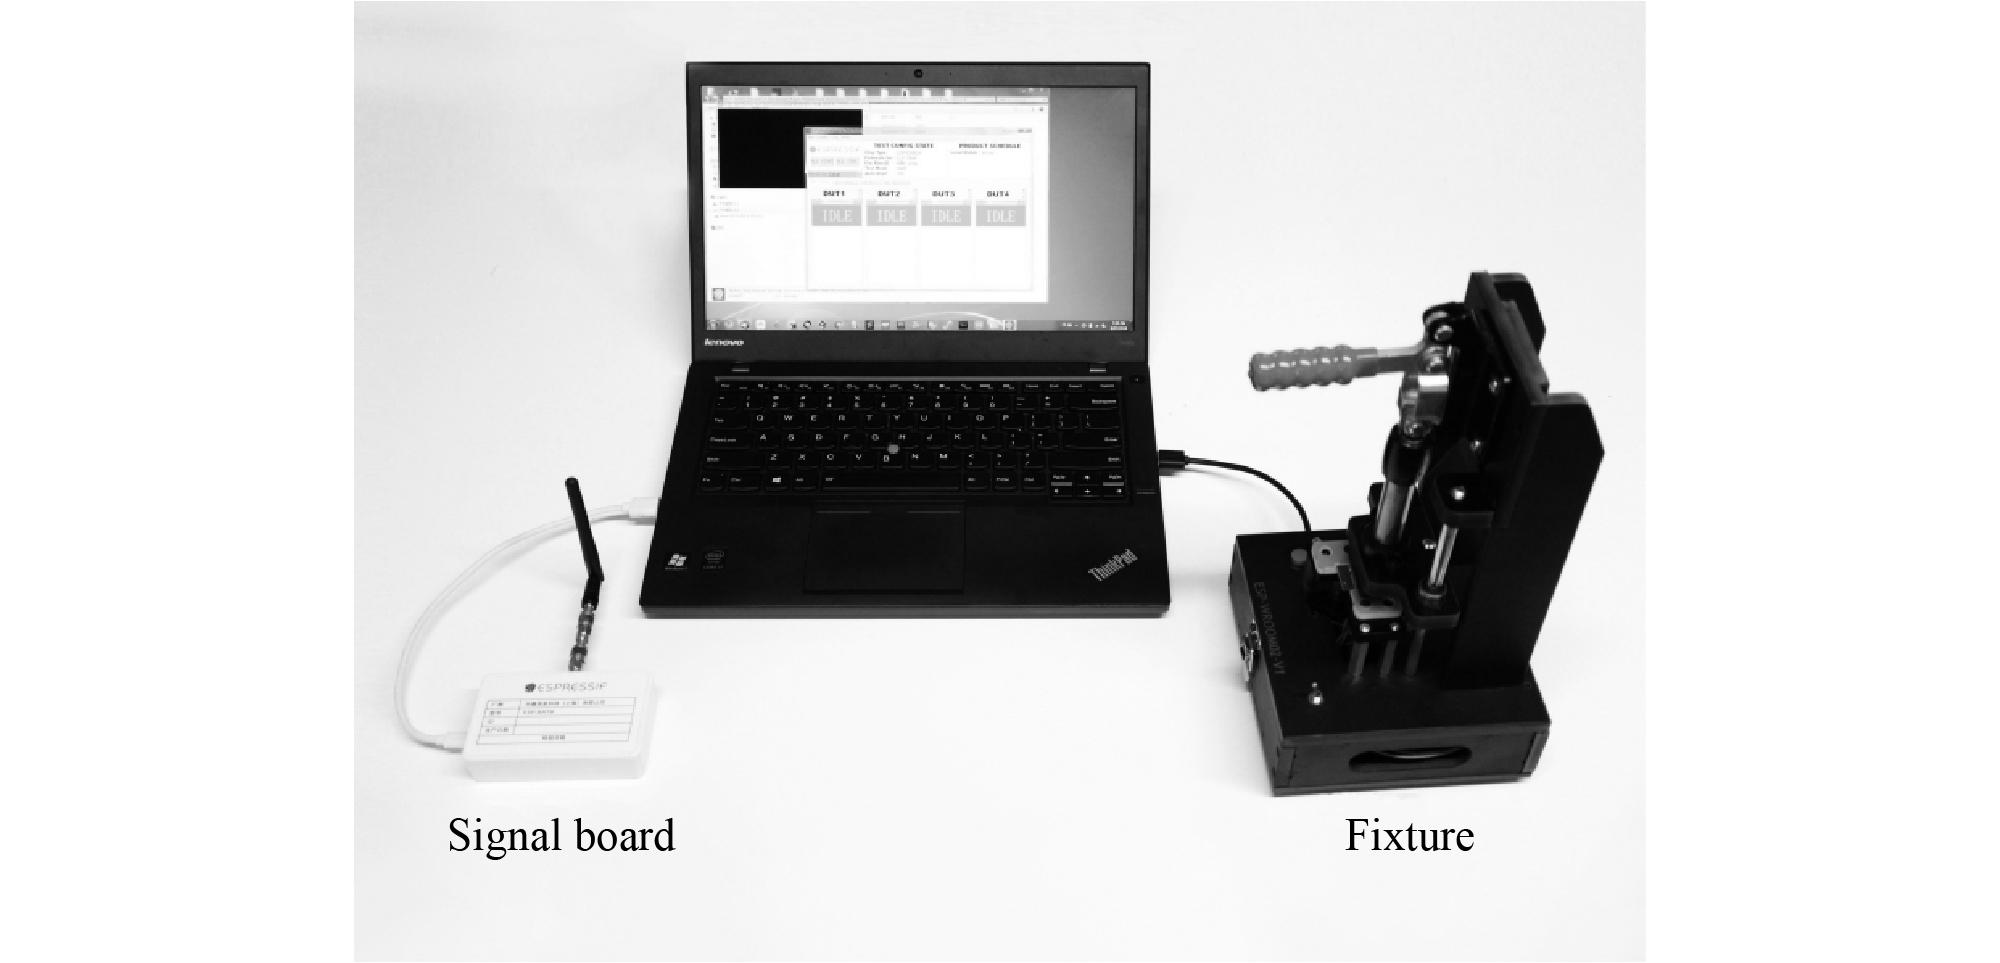
\includegraphics[width=\textwidth]{D14Z/14-5}
    \caption{\Centering\newline Hardware connection for signal board scheme}
  \end{minipage}
\end{figure}

\section{Practice: Mass Production Data in Smart Light Project}

In the Smart Light project introduced in this book, each device needs to store some unique information for identification, as well as some common configuration for operation. The public ESP RainMaker used in the project is for prototyping and evaluation, which only allows adding five devices at most. You can generate binary files of mass production data based on obtained credentials and modify relevant source codes to stimulate the operations in mass production. To get the Cloud connectivity credentials of a larger scale, please contact Espressif for private ESP RainMaker deployments.

\section{Summary}

In this chapter, we introduced the mass production testing of products based on Espressif's modules and chips, and the burning of mass production firmware, so that readers can have a preliminary understanding of mass production. For devices to be identified and bound to users, unique mass production data must be burned to each device. To save manufacturers’ trouble of burning firmware in mass production, Espressif provides modules with customized firmware, which can be mounted directly onto the product’s hardware circuit.

\end{document}